\documentclass[a4paper, 14pt]{extreport}
\usepackage{cmap}
\usepackage{amssymb}
\usepackage{amsmath}
\usepackage{graphicx}
\usepackage{amsthm}
\usepackage{upgreek}
\usepackage{listings}
\usepackage{mathtools}
\usepackage{setspace}
%\numberwithin{equation}{section}
\usepackage[T2A]{fontenc}
\usepackage[utf8]{inputenc}
\usepackage[normalem]{ulem}
\usepackage{mathtext} % русские буквы в формулах
\usepackage[left=3cm,right=1cm,top=2cm,bottom=2cm]{geometry}
\usepackage{indentfirst}
\usepackage{linegoal}
\usepackage[english,russian]{babel}
\usepackage[unicode]{hyperref}
\newcommand\Norm[1]{\left\| #1 \right\|}
\newcommand{\dif}{\mathrm{d}}
\newcommand{\Rm}{\mathbb{R}}
\newcommand{\Cm}{\mathbb{C}}
\newcommand{\Z}{\mathbb{Z}}
\newcommand{\I}{\mathbb{I}}
\newcommand{\N}{\mathbb{N}}
\newcommand{\rank}{\operatorname{rank}}
\newcommand{\Ra}{\Rightarrow}
\newcommand{\ra}{\rightarrow}
\newcommand{\FI}{\Phi}
\newcommand{\Sp}{\text{Sp}}
\renewcommand{\leq}{\leqslant}
\renewcommand{\geq}{\geqslant}
\renewcommand{\beta}{\upbeta}
\renewcommand{\gamma}{\upgamma}
\renewcommand{\delta}{\updelta}
\renewcommand{\varphi}{\upvarphi}
\renewcommand{\tau}{\uptau}
\renewcommand{\sigma}{\upsigma}
\renewcommand{\lambda}{\uplambda}
\renewcommand{\psi}{\uppsi}
\renewcommand{\mu}{\upmu}
\renewcommand{\omega}{\upomega}
\renewcommand{\d}{\operatorname{d}}
\renewcommand{\xi}{\upxi}
\renewcommand{\epsilon}{\upvarepsilon}
\newcommand{\Binom}{\operatorname{Binom}}
\newcommand{\Pois}{\operatorname{Pois}}
\newtheorem*{theorem}{Теорема}
\newtheorem*{cor}{Следствие}
\newtheorem*{lem}{Лемма}
\usepackage{stackengine}


%%%%%%%%%%%%%%%%%%%%%%%%%%%%%%%%%%%%%%%%%%%%%%%%%%%%%%%%%%%%%%%%%%%%%%%%%%%
% РИСУНКИ
%%%%%%%%%%%%%%%%%%%%%%%%%%%%%%%%%%%%%%%%%%%%%%%%%%%%%%%%%%%%%%%%%%%%%%%%%%%%

\newcounter{figcount}[chapter]
\renewcommand{\thefigcount}{\arabic{chapter}.\arabic{figcount}}
\newcommand{\dfig}[1]%
{\refstepcounter{figcount}\rm \small \bf Рисунок \thefigcount \ --- \  #1}



%%%%%%%%%%%%%%%%%%%%%%%%%%%%%%%%%%%%%%%%%%%%%%%%%%%%%%%%%%%%%%%%%%%%%%%%%%%
%  СОДЕРЖАНИЕ
%%%%%%%%%%%%%%%%%%%%%%%%%%%%%%%%%%%%%%%%%%%%%%%%%%%%%%%%%%%%%%%%%%%%%%%%%%%%


\addto\captionsrussian{\def\contentsname{\centerline{ОГЛАВЛЕНИЕ\vspace{-1em}}}}
\setcounter{tocdepth}{1}

\RequirePackage{titletoc}

\titlecontents{chapter}[0pt]{\vspace{1em}}{\bfseries ГЛАВА \contentslabel{0em} \hspace*{0.5em}}
{\bfseries}{\titlerule*[1pc]{.}\contentspage}


\titlecontents{section}[0pt]{}{\thecontentslabel \quad }
{}{\titlerule*[1pc]{.}\contentspage}



\begin{document}
	\def\contentsname{ОГЛАВЛЕНИЕ}
	
	  \begin{titlepage}
		\begin{center}
			\textbf{БЕЛОРУССКИЙ ГОСУДАРСТВЕННЫЙ УНИВЕРСИТЕТ
				\\[5mm]
				{ФАКУЛЬТЕТ ПРИКЛАДНОЙ МАТЕМАТИКИ И ИНФОРМАТИКИ}\\[2mm]
				Кафедра математического моделирования и анализа данных
			}
			
			\vfill
			
			\textbf{Отчет
				\\[3mm]
				о прохождении производственной (преддипломной) практики
				\\[26mm]
			}
		\end{center}
		
		\hfill
		\begin{minipage}{.6\textwidth}
			\begin{flushright}
				Гут Валерии Александровны\\
				студентки 4 курса 7 группы\\
				специальности «Прикладная математика»\\[5mm]
				
				Руководитель практики:\\[2mm] 
				старший преподаватель\\
				кафедры математического моделирования\\
				и анализа данных ФПМИ,\\
				С.В.Лобач\\
				
				
			\end{flushright}
		\end{minipage}
		\vfill
		\begin{center}
			Минск, 2025\ г.
		\end{center}
	\end{titlepage}
	\newpage
	\setcounter{page}{2}
	\begin{center}
		{
			\setstretch{0.5}
			\mbox{БЕЛОРУССКИЙ~ГОСУДАРСТВЕННЫЙ~УНИВЕРСИТЕТ} \\~\\
			\mbox{Факультет~прикладной математики~и~информатики} \\~\\
			\mbox{Кафедра~математического~моделирования~и~анализа~данных} \\~\\[2mm]
		}
		\vspace{0.5cm}
		\hfill
		\begin{minipage}{.6\textwidth}
			\begin{flushright}
				\textbf{Утверждаю}\hspace*{4.2cm} \\
				Заведующий кафедрой \underline{\hspace*{4cm}}\\[-2mm]
				{\scriptsize(подпись)(фамилия, инициалы)}\\[2ex]
				«\underline{\hspace*{0.5cm}}»\underline{\hspace*{2cm}}20\underline{\hspace*{0.5cm}}г.
				
			\end{flushright}
		\end{minipage}
		
		\vspace{1cm}
		\bf
		{
			\mbox{Задание на практику}\\
			\mbox{по специальности «Прикладная математика»} \\[6mm]
		}
	\end{center}
	Студентке Гут В. А.\\[2mm]
	1. Тема практики:
	<<Статистический анализ моделей распространения заболеваний>>.\\[6mm]
	2. Список рекомендуемой литературы:
	
	2.1. Statistical forecasting of the dynamics of epidemiological indicators for COVID-19 incidence in the Republic of Belarus / Yu. S. Kharin, V. A. Valoshka, O. V. Dernakova, V. I. Malugin, A. Yu. Kharin// Journal of the Belarusian State University. Mathematics and Informatics. - 2020. - № 3. - С. 36-50
	
	2.2. Детерминированные и стохастические модели распространения инфекции и тестирование в изолированном контингенте/ Чигарев, А. В.,Журавков, М. А.,Чигарев, В. А.// Журнал Белорусского государственного университета. Математика.
	
	2.3. Lazzizzera, I. (2021) An Analytic Approximate Solution of the SIR Model. Applied Mathematics, 12, 58-73
	
	2.4. МАТЕМАТИЧЕСКАЯ ЭПИДЕМИОЛОГИЯ Учебно–методическое пособие
	по выполнению лабораторных работ / В. Н. Леоненко // УНИВЕРСИТЕТ ИТМО Санкт–Петербург. -- 2018. С. 10-30.\\[6mm]
	3. Перечень подлежащих разработке вопросов или краткое содержание
	расчетно-пояснительной записки:
	
	3.1. изучение рекомендованной литературы;
	
	3.2. изучение предложенных в литературе алгоритмов;
	
	3.3. компьютерная реализация алгоритмов;
	
	3.4. сравнение алгоритмов;
	
	3.5. подготовка отчета и презентации.\\[6mm]
	4. Примерный календарный график:\\[6mm]
	
	-- \textbf{февраль (1-ая неделя)} -- получение задания, ознакомление с условиями работы, изучение основных теоретических вопросов;
	
	-- \textbf{февраль (2-3-я неделя)} -- вывод базовой дифференциальной модели SIR и ее модификаций для симуляции процесса распространения заболеваний; описание преимуществ моделей
	
	-- \textbf{март (4-5-ая неделя)} -- изучение и математическое описание вероятностных популяционных моделей и имитационных моделей с пространственной структурой;
	
	-- \textbf{март (6-7-ая неделя)} -- изучение и описание индивидуум - ориентированных и мультиагентных методов моделирования; описание решаемой прикладной задачи, построение детерминированной модели распространения заболеваний;
	
	-- \textbf{апрель (8-9-ая неделя)} -- построение вероятностной, пространственной и мультиагентной моделей распространения заболеваний; подведение итогов;
	
	
	-- \textbf{апрель (10-ая неделя)} -- описание, оформление теоретической части работы; подготовка презентации.\\[6mm]
	5. Руководители практики:
	
	от предприятия Николайчик Марина Александровна;
	
	от кафедры Лобач Сергей Викторович.\\[6mm]
	6. Дата выдачи задания 10.02.2025.\\[6mm]
	7. Срок сдачи отчета\hspace*{0.7cm} 21.04.2025.\\[10mm]
	Руководитель \underline{\hspace*{4cm}} С. В. Лобач\\[-2mm]
	{\scriptsize(от кафедры)\hspace*{1.5cm}(подпись)}\\[2ex]
	\noindent Подпись студента \underline{\hspace*{6cm}} \\[-2mm]
	{\scriptsize\hspace*{6cm}(подпись, дата)}\\[2ex]
	\newpage
	
	
	% Содержание
	\tableofcontents
	\newpage
	\chapter*{ВВЕДЕНИЕ}\addcontentsline{toc}{chapter}{ВВЕДЕНИЕ}
	Математические методы для анализа заболеваний впервые были использованы Даниэлем Бернулли в 1760 году, когда он оценивал эффективность различных методов вакцинации против оспы. В 1840 году Уильям Фарр описал статистику смертности от оспы в Англии и Уэльсе за 1837-1839 годы, применив кривую нормального распределения. Этот подход был усовершенствован Джоном Браунли, который в 1906 году опубликовал статью «Статистический подход к иммунной защите: теория эпидемий», в которой сопоставлял эпидемиологические данные, используя распределение Пирсона. Также в это время Хамер и Росс начали применять математическое описание распространения заболеваний, что помогло прояснить механизмы повторения эпидемии кори и связь между числом комаров и малярией. Их работы, наряду с исследованиями Росса, Хадсона, Сопера и Кермака с Маккендриком, стали основой для дальнейших исследований в области математического моделирования эпидемий.
	
	В этих работах впервые был использован «закон действующих масс», утверждающий, что число новых инфекций пропорционально произведению чисел восприимчивых и инфицированных. Модель Кермака и Маккендрика положила начало популярности SIR-моделей, описывающих динамику восприимчивых, инфицированных и выздоровевших через системы дифференциальных или разностных уравнений.
	
	SIR (Susceptible Infections Recovered) модель, описывающая распространение эпидемии, является базовой при применении подходов математического моделирования, так как включает в себя в простейшем варианте основные фазы эпидемии и, в тоже время, допускает их уточнение на основе корректирующих членов в уравнениях, а также добавления в систему  исходных разрешающих уравнений новых уравнений. 
	SIR-модель удобно использовать для модификации детерминированного подхода в вероятностный, так как она учитывает тот факт, что эпидемиологические процессы протекают в условиях наличия неполной информации и погрешностей наблюдения.
	
	В начале 1920-х годов стало очевидно, что для малых групп населения, таких как семьи, вероятностное описание эпидемий более эффективно. В 1926 году Маккендрик предложил стохастическую версию SIR-модели для анализа продолжительности эпидемий гриппа и малярии, хотя его работа не была сразу признана. Важное влияние на модели с вероятностным описанием оказали исследования Гринвуда и модель Рида и Фроста, которые использовали биномиальные распределения, что дало начало термину «цепочечно-биномиальные модели».
	
	Однако еще в 1889 году российский врач-эпидемиолог Петр Дмитриевич Енько представил модель распространения инфекционных заболеваний в дискретном времени, описывающую средние значения по модели Рида и Фроста. Его работа стала известна благодаря обзору Клауса Дитца и Дитера Шенцле о математических моделях в эпидемиологии. Позже они обсудили возможности обобщения модели Енько с использованием различных законов распределения для контактов. Публикация Енько была переведена на английский язык в 1989 году, и его признали первым специалистом по моделированию эпидемий.
	
	Исследования стохастической SIR-модели, опубликованные Бартлеттом в 1949 году, стали основой для развития стохастических моделей эпидемий. Позже, работы Бейли и Уиттла значительно обогатили применение теории случайных процессов в этой области.
	
	В 1957 году Кендалл предложил одну из первых пространственных моделей эпидемий, основанную на уравнениях в частных производных. В том же году Бартлетт исследовал распространение заболеваний на узлах пространственной структуры 6×6 с использованием методов имитационного моделирования. В 1971 году Фокс и Элвбэк представили первую индивидуум-ориентированную модель распространения заболеваний. Однако новое направление не сразу получило признание из-за недостатка данных и низкой производительности компьютеров.
	
	В 80-х годах началось активное развитие математических моделей для оценки методов борьбы с раком, включая массовые обследования. Эти модели разрабатывались как на основе детерминированных, так и вероятностных подходов. Быстрый прогресс вычислительных технологий в 80-90-х годах позволил полноценно использовать стохастические модели, что вызвало интерес к индивидуум-ориентированному моделированию заболеваний в разнообразных популяциях на стыке XX и XXI веков.
	
	В качестве рассматриваемого заболевания мы выберем распространение гриппа в Беларуси. Ежегодно в Республике Беларусь в период с октября по апрель отмечается сезонный подъем заболеваемости острыми респираторными инфекциями, в том числе гриппом. В настоящее время интенсивность эпидемического процесса ОРВИ оценивается как средняя с тенденцией к увеличению во всех регионах республики. В структуре заболевших удельный вес детского населения в возрасте до 18 лет составляет более 50\%. Таким образом, собрав необходимые для моделирования данные о протекании гриппа по Беларуси, мы построим популяционные модели распространения гриппа, что позволит нам нагляднее рассмотреть исследуемые модели.
	
	
	\newpage
	\chapter{МОДЕЛИРОВАНИЕ ПРОЦЕССА РАСПРОСТРАНЕНИЯ ГРИППА}
	\section{Постановка практической задачи}
	Сформулируем практическую задачу. Необходимо смоделировать процесс распространения гриппа. Для этого нам нужно собрать всю необходимую для моделирования информацию о распространении гриппа.
	
	Грипп -- это острое респираторное вирусное заболевание, вызываемое вирусами гриппа и поражающее в первую очередь верхние дыхательные пути, а также бронхи и, в более редких случаях, -- лёгкие. Выделяется среди острых респираторных вирусных инфекций у людей из-за возможного тяжёлого течения болезни. Грипп ассоциируется с высокой смертностью во время пандемий, эпидемий и спорадических вспышек. Пандемии гриппа случаются примерно каждые 50 лет, эпидемии же наблюдаются чаще. Вспышки сезонного гриппа ежегодно происходят почти во всём мире. Наиболее частой причиной сезонного гриппа являются вирусы гриппа A, также только эти вирусы гриппа известны как причина пандемий.
	
	Симптомы гриппа появляются на 1—4-й день после заражения и включают в себя лихорадку, кашель, головную боль, боль в мышцах и суставах, слабость, боль в горле и насморк. При этом кашель может длиться две и более недели. Наиболее заразен больной на 3—4-й день с момента появления симптомов. Реконвалесцентный период составляет 7—15 дней.[7] После выздоровления формируется иммунитет к конкретному штамму вируса, но он не защищает от других штаммов. Иммунитет носит временный характер (обычно до 1-2 лет).
	
	Индекс репродукции ($R_{0}$, в медицинской литературе часто базовое репродуктивное число; также базовый показатель репродукции) -- это безразмерный параметр, характеризующий заразность инфекционного заболевания в медицинской и ветеринарной эпидемиологии. Обычно определяется как количество людей, которые будут заражены типичным заболевшим, попавшим в полностью неиммунизированное окружение при отсутствии специальных эпидемиологических мер, направленных на предотвращение распространения заболевания (например, карантина). Если $R_0 > 1$. то на начальном этапе число заболевших будет расти экспоненциально.[8]
	
	Для гриппа будем считать, что базовое репродуктивное число для гриппа 0.9-2.1. Тогда в качестве базового репродуктивного числа возьмем среднее значение $$R_0 = 1.5.$$
	\section{Формулировка детерминированной SEIR модели}
	Пусть определено некоторое множество $T \subset \mathbb R$, которое задает некоторый временной промежуток. И пусть также
	\begin{itemize}
		\item $t \in T$ --- независимая переменная, обозначающая некоторый момент времени;
		\item $N \in \mathbb R$ --- общая численность населения.
	\end{itemize}
	Очень часто стандартная модель SIR является слишком простой и
	нереалистичной, так как в ней полагается, что особь является заразной сразу же после инфицирования. В SEIR модели предполагается, что инфекция имеет инкубационный период, в течение которого люди инфицированы, но
	еще не заразны. Эта группа людей обозначается через $E$ (exposed). С учетом нового класса получаем следующую структуру
	популяции:
	$$S + E + I + R = N,$$ где
	\begin{itemize}
		\item $S(t)$ -- это количество не инфицированных людей. Причем скорость изменения количества подверженных зависит от вероятности передачи инфекции, количества инфицированных и количества подверженных, где $\beta$ -- это скорость передачи заболевания;
		\item $E(t)$ -- это число инфицированных, но еще не заразных людей. Причем скорость изменения количества инфицированных, но еще не заразных людей зависит от входящего потока людей, проходящих инкубационный период, а также выходящего потока этих же людей. Параметр $\sigma^{-1}$ представляет собой среднюю продолжительность инкубационного периода;
		\item $I(t)$ -- это количество инфицированных людей. Причем	скорость изменения количества инфицированных зависит от входящего потока инфицированных и выходящего потока инфицированных. Параметр $\gamma$ -- это скорость восстановления;
		\item $R(t)$ -- это группа выздоровевших лиц, а именно людей, которые восстановились.
	\end{itemize}
	Модель SEIR описывается задачей Коши
	\begin{equation}
		\label{seir}
		\begin{dcases}
			\dfrac {\d S(t)}{\d t} = - \beta \cdot I(t)\cdot S(t),\\
			\dfrac {\d E(t)}{\d t} = \beta \cdot S(t)\cdot I(t) - \sigma\cdot E(t),\\
			\dfrac{\d I(t)}{\d t} =\sigma \cdot E(t) - \gamma\cdot I(t),\\
			\dfrac{\d R(t)}{\d t} = \gamma\cdot I(t),\\
			S(0) = S_0,\ I(0) = I_0,\ E(0) = 0,\ R(0) = 0.
		\end{dcases}
	\end{equation}
	
	Схематически эта модель может быть записана в следующем виде (Рисунок \ref{fig6})
	\begin{figure}[h!]
		\center{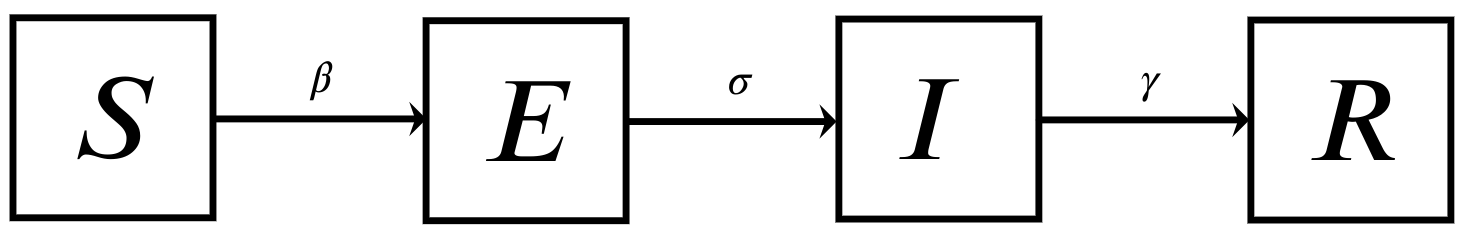
\includegraphics[scale=0.25]{images/img08}}
		
		\dfig{Схема перехода индивидов модели SEIR}\label{fig6}
	\end{figure}
	
	
	Важно отметить, что модель SEIR является упрощенной моделью и не учитывает множество реальных факторов, таких как вакцинация, мутации вируса и изменение поведения людей. Но она предоставляет базовый фреймворк для изучения распространения инфекции и позволяет прогнозировать общую динамику эпидемии.
	Именно на примере этой модели мы и будем проводить эксперименты в главе 3.
	
	Дополнительные вариации модели SEIR также могут включать дополнительные факторы, такие как иммунизация или введение противоэпидемических мер. Модель SEIR и ее вариации широко используются в исследованиях эпидемиологии и планировании общественного здравоохранения. Они позволяют ученым и решающим органам оценить различные стратегии контроля эпидемии, такие как вакцинация, социальное дистанцирование, использование масок и карантинные меры. Такие модели могут помочь прогнозировать будущие тенденции распространения болезни и определить наиболее эффективные меры по сдерживанию инфекции.
	
	Для того, чтобы построить приближенное численное решение задачи Коши 
	\eqref{seir}, можно использовать классические численные методы интегрирования обыкновенных дифференциальных уравнений. К примеру, метод Эйлера, методы Рунге-Кутты, методы предиктор-корректора.
	
	В частности мы будем использовать пакет scipy из Python, в котором предложен алгоритм LSODE (алгоритм Ливермора для обыкновенных дифференциальных уравнений), который решает жесткие и нежесткие системы дифференциальных уравнений первого порядка. В нежестком случае используются методы Адамса (методы предиктор-корректора), а в жестком случае -- методы обратной дифференциации (BDF) (методы Гира). Линейные системы, которые возникают, решаются прямыми методами (LU-факторизация).
	
	Таким образом, вдаваться в формальное представление итерационных алгоритмов численного решения мы не будем. 
	
	\section{Применение детерминированной SEIR модели для моделирования}
	На основе приведенной информации о распространении можем сформулировать математическую модель следующим образом. Так как симптомы появляются через 1-4 дня, то возьмем средний инкубационный период для модели $T_\text{инкубац} = 2$ дня. Тогда коэффициент перехода из $E$ в $I$ равна
	$$\sigma = \dfrac{1}{T_\text{инкубац}} = \dfrac 1 2 = 0.5.$$
	Средний инфекционный период выберем $T_\text{инфекц}=5$ дней.
	Тогда коэффициент выздоровления равен
	$$\gamma = \dfrac{1}{T_\text{инфекц}} = \dfrac 1 5 = 0.2.$$
	Коэффициент передачи инфекции $\beta$ мы можем получить из  базового репродуктивного числа через следующее соотношение
	$$\beta = R_0\cdot \gamma = 1.5\cdot 0.2 = 0.3.$$
	
	В качестве числа населения возьмем $N=1000$, а число инфицированных зададим равное $I_0 = 20$. Отсюда $S_0 = N - I_0 = 980$. Данный процесс будем рассматривать в течение $T=100$ дней.
	
	Таким образом, мы можем описать процесс распространения гриппа с помощью классической SEIR модели
	\begin{equation*}
		\begin{dcases}
			\dfrac {\d S(t)}{\d t} = - 0.3 \cdot I(t)\cdot S(t),\\
			\dfrac {\d E(t)}{\d t} = 0.3 \cdot S(t)\cdot I(t) - 0.5\cdot E(t),\\
			\dfrac{\d I(t)}{\d t} =0.5 \cdot E(t) - 0.2\cdot I(t),\\
			\dfrac{\d R(t)}{\d t} = 0.2\cdot I(t),\\
			S(0) = 980,\ I(0) = 20,\ E(0) = 0,\ R(0) = 0.
		\end{dcases}
	\end{equation*} 
	
	Приведем график численного решения поставленной задачи Коши
	
\begin{figure}[h!]
	\center{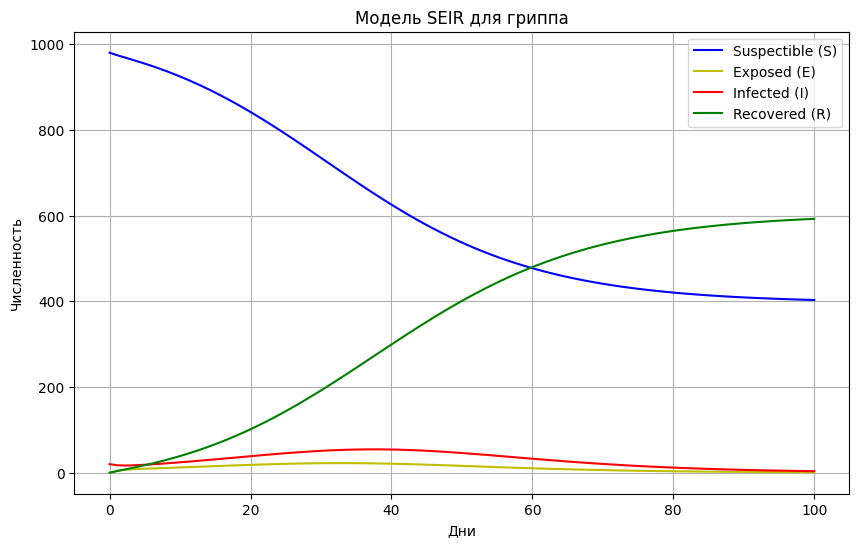
\includegraphics[width=\textwidth]{images/graph01}}
	
	\dfig{График численного решения задачи Коши для детерминированной SEIR модели}\label{graph01}
\end{figure}
	
	Из графика видно, как сперва число здоровых людей начинает стремительно уменьшатся, пока не достигает грани в 400. Число выздоровевших же напротив начинает стремительно возрастать, пересекается с график числа здоровых людей на 60-ый день, а затем скорость становится все ниже и ниже, пока не достигается грань в 600 человек. Как можно видеть, через 100 дней после начала эпидемии число болеющих практически снизилось до нуля. То есть мы можем заключить, что приблизительно спустя 100 дней эпидемия прекратилась.
	\section{Применение вероятностной SEIR модели для моделирования}
	Построим вероятностную модель с дискретным временем, поскольку для нее легко привести численную реализацию. Вероятностная SEIR-модель для гриппа имеет следующий вид
	\begin{equation}
		\begin{dcases}
			S_{t+1} = S_t - \Delta E_t,\\
			E_{t+1} = E_t +\Delta E_t - \Delta I_t,\\
			I_{t+1} = I_t + \Delta I_t - \Delta R_t,\\
			R_{t+1} = R_t + \Delta R_t,
			S_0 = 980,\ E_0 = 0,\ I_0 = 20,\ \ R_0 = 0
		\end{dcases}
		t = 0,1,2\ldots,
	\end{equation}
	при этом
	$$\Delta E_t \sim \Binom\left(S_t, 
	1 - \exp\left(-\beta\cdot  \frac{I}{N} \cdot \Delta t\right)\right),$$
	$$\Delta I_t \sim \Binom\left(E_t, 1 - \exp\left(-\sigma \cdot \Delta t\right)\right),$$
	$$\Delta R_t \sim \Binom\left(I_t, 1 - \exp\left(-\gamma \cdot \Delta t\right)\right).$$
	
	Таким образом, мы можем описать процесс распространения гриппа с помощью вероятностной SEIR модели. Приведем 100 реализаций этой модели, а в качестве результирующего графика выберем средние значения для каждой группы, а также приведем 95\%-доверительные интервалы для каждой переменной
	
	\begin{figure}[h!]
		\center{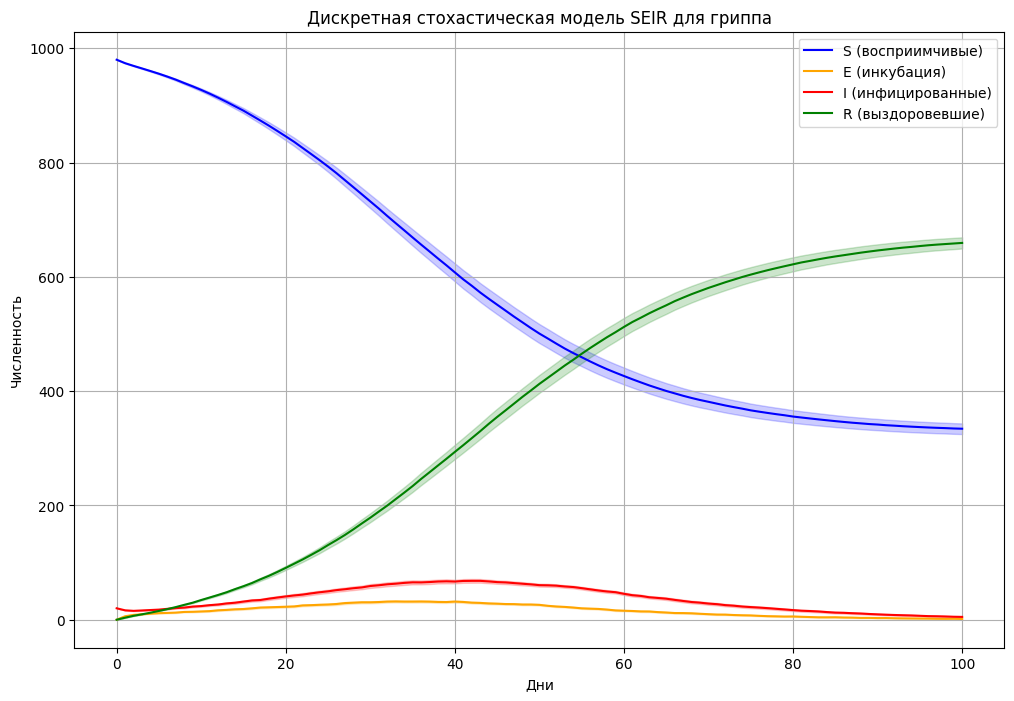
\includegraphics[width=\textwidth]{images/graph02}}
		
		\dfig{График численной реализация вероятностной SEIR для гриппа с доверительными интервалами}\label{graph02}
	\end{figure}
	
	Из графика видно, что поведения функций, описывающих группы людей, не сильно изменились относительно детерминированного случая. Однако теперь сместились границы, при которых число восприимчивых людей перестает снижаться, а число выздоровевших -- расти. 
	
	\section{Применение пространственной SEIR модели для моделирования}
	Для пространственной модели построим сетку узлов $30 \times 30$ на которой зададим вероятностную SEIR-модель для дискретного времени с сохранением всех параметров из предыдущего случая. Клетки, в которых будут находиться инфицированные люди, будут выбираться случайно.
	
	Таким образом, мы можем описать процесс распространения гриппа с помощью вероятностной SEIR-модели в пространстве. Приведем на графике одну из реализаций через каждые 10 дней
	
	\begin{figure}[h!]
		\center{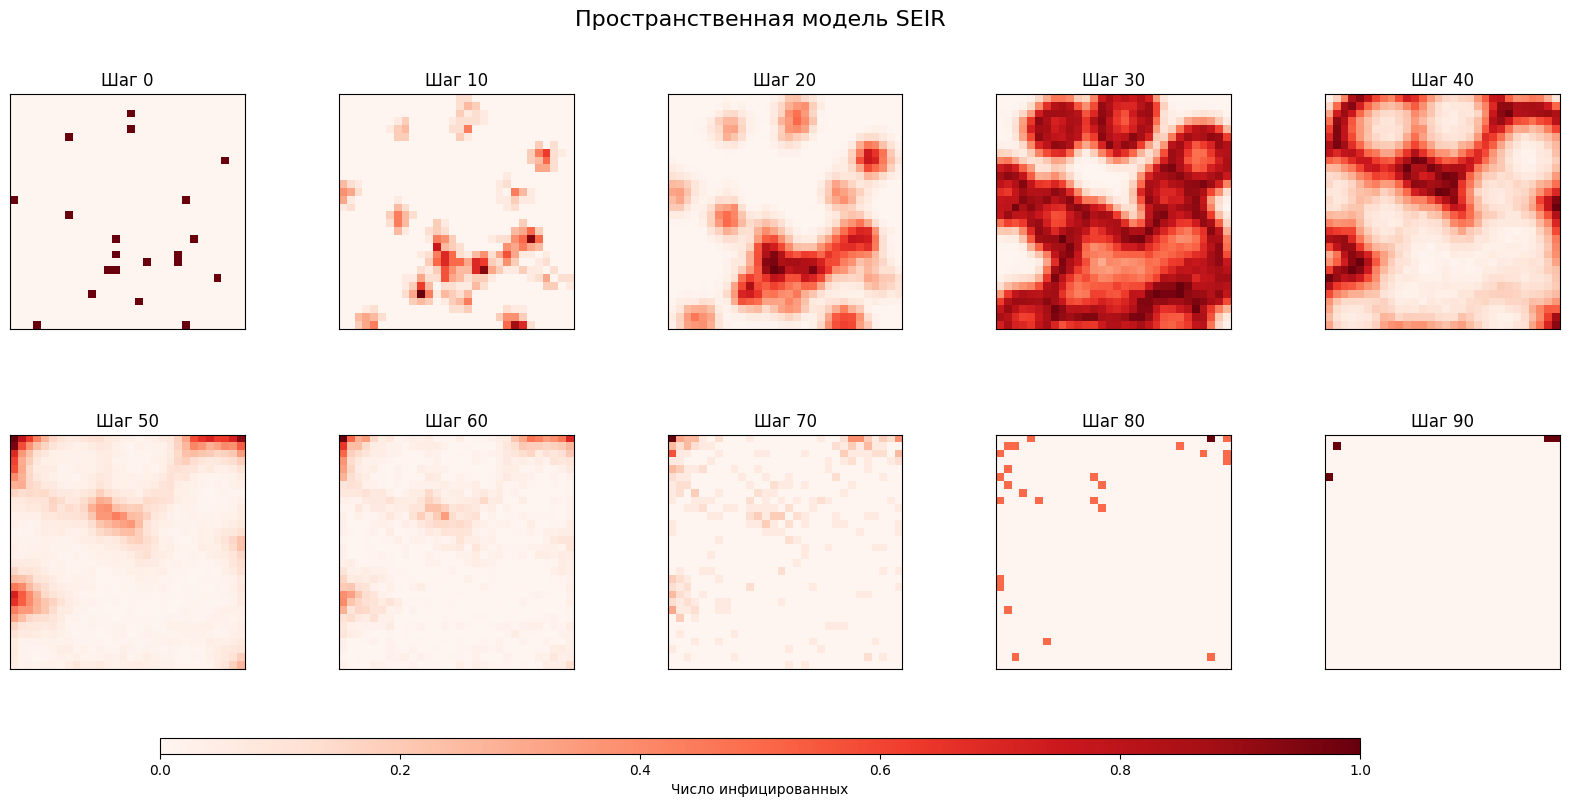
\includegraphics[width=\textwidth]{images/graph03}}
		
		\dfig{Пространственные графики численной реализации вероятностной SEIR модели для гриппа}\label{graph03}
	\end{figure}
	
	Из построенных графиков видно, что, как и в предыдущих случаях, спустя 30-40 дней число инфицированных особей достигает своего пика, а затем стремительно снижается до такой степени, что уже на 90-ый день число инфицированных стремится к нулю. Кроме этого также заметно, как все эти изменения отражаются в пространстве.
	
	\section{Применение мультиагентной SEIR модели для моделирования}
	Алгоритм моделирует распространение инфекции в популяции агентов, используя модифицированную модель SEIR (восприимчивые, экспонированные, инфицированные, выздоровевшие). Популяция агентов размещена в двумерном пространстве, и их поведение включает перемещение, заражение и смену состояния в зависимости от времени и контактов с другими агентами. Графики показывают динамику агентов на разных временных шагах.
	
	\subsubsection*{Шаг 1}
	
	На первом этапе создаётся популяция агентов с заданными свойствами:
	
	\begin{itemize}
		\item {Количество агентов ($N_{\text{agents}}$)}: Всего агентов в симуляции.
		\item {Позиции агентов}: Каждый агент случайным образом размещается в двумерном пространстве размера $L \times L$.
		\item {Индивидуальные параметры агентов}: Для каждого агента задаются случайные значения:
		\begin{itemize}
			\item {Восприимчивость ($\text{susceptibility}$)}: Коэффициент, влияющий на вероятность заражения.
			\item {Интенсивность контактов ($\text{contact\_rate}$)}: Сколько контактов совершает агент.
			\item {Инкубационный период ($\text{incubation\_period}$)}: Время, необходимое для перехода из состояния <<Экспонированный>> (E) в <<Инфицированный>> (I).
			\item {Инфекционный период ($\text{infectious\_period}$)}: Время, через которое инфицированный агент выздоравливает.
		\end{itemize}
		\item {Начальное состояние}: Большинство агентов находятся в состоянии <<Восприимчивые>> (S). Несколько агентов (определяется параметром\\ initial\_infected) изначально заражены (I).
	\end{itemize}
	
	\subsubsection*{Шаг 2}
	
	На каждом временном шаге ($T$) выполняются следующие действия для обновления состояния агентов:
	
	\begin{enumerate}
		\item Перемещение агентов
		\begin{itemize}
			\item Каждый агент с заданной вероятностью ($\text{move\_prob}$) перемещается случайным образом в пределах пространства.
			\item Если агент выходит за границы пространства, его позиция корректируется (ограничивается рамками пространства $L \times L$).
		\end{itemize}
		\item Обновление состояния агента
		\begin{itemize}
			\item {Если агент в состоянии <<Экспонированный>> (E)}:
			\begin{itemize}
				\item Увеличивается таймер заражения ($\text{time\_infected}$).
				\item Если время заражения превышает инкубационный период, агент переходит в состояние <<Инфицированный>> (I).
			\end{itemize}
			\item {Если агент в состоянии <<Инфицированный>> (I)}:
			\begin{itemize}
				\item Также увеличивается таймер заражения ($\text{time\_infected}$).
				\item Если таймер превышает инфекционный период, агент переходит в состояние <<Выздоровевший>> (R).
			\end{itemize}
		\end{itemize}
		\item Заражение других агентов
		\begin{itemize}
			\item Если агент находится в состоянии <<Инфицированный>> (I), он может заразить других агентов, находящихся рядом (расстояние меньше 0.5).
			\item Вероятность заражения определяется формулой:
			\[
			P_{\text{infect}} = \beta \cdot \text{susceptibility},
			\]
			где $\beta$~--- коэффициент передачи инфекции.
			\item Если случайное число меньше $P_{\text{infect}}$, агент в состоянии <<Восприимчивый>> (S) переходит в состояние <<Экспонированный>> (E), и его таймер заражения сбрасывается.
		\end{itemize}
	\end{enumerate}
	
	\subsubsection*{Шаг 3}
	
	Каждые 10 временных шагов (или другой заданный интервал) сохраняется:
	\begin{itemize}
		\item Текущее состояние всех агентов.
		\item Время ($t$), соответствующее этому состоянию.
	\end{itemize}
	
	Эти данные используются для построения графиков.
	
	\subsubsection*{Шаг 4}
	
	Создаётся сетка из графиков, отображающих положение агентов в пространстве на разных временных шагах. Каждый график отражает состояние популяции в конкретный момент времени.
	
	{Цветовое кодирование состояния агентов}:
	\begin{itemize}
		\item {Синий (S)}~--- восприимчивые агенты.
		\item {Оранжевый (E)}~--- экспонированные агенты.
		\item {Красный (I)}~--- инфицированные агенты.
		\item {Зелёный (R)}~--- выздоровевшие агенты.
	\end{itemize}
	
	\subsubsection*{Используемые параметры и их влияние}
	
	\begin{itemize}
		\item {$N_{\text{agents}}$}~--- количество агентов:
		\begin{itemize}
			\item Чем больше агентов, тем плотнее популяция, что может ускорить распространение инфекции.
		\end{itemize}
		\item \textbf{$L$}~--- размер пространства:
		\begin{itemize}
			\item Чем больше пространство, тем сложнее агентам контактировать, что замедляет заражение.
		\end{itemize}
		\item \textbf{$\beta$}~--- коэффициент передачи:
		\begin{itemize}
			\item Определяет вероятность заражения при контакте. Чем выше, тем быстрее распространяется инфекция.
		\end{itemize}
		\item {$\sigma_{\text{mean}}$ и $\gamma_{\text{mean}}$}~--- инкубационный и инфекционный периоды:
		\begin{itemize}
			\item Увеличение этих параметров замедляет переход между состояниями, что влияет на динамику эпидемии.
		\end{itemize}
		\item {$\text{move\_prob}$}~--- вероятность перемещения агентов:
		\begin{itemize}
			\item Чем больше значение, тем чаще агенты перемещаются, что увеличивает вероятность контактов и заражения.
		\end{itemize}
		\item {$\text{initial\_infected}$}~--- начальное число заражённых:
		\begin{itemize}
			\item Определяет начальный уровень инфекции. Чем больше заражённых в начале, тем быстрее эпидемия распространяется.
		\end{itemize}
	\end{itemize}
	
	Приведем графический результат работы алгоритма
	
	\begin{figure}[h]
		\center{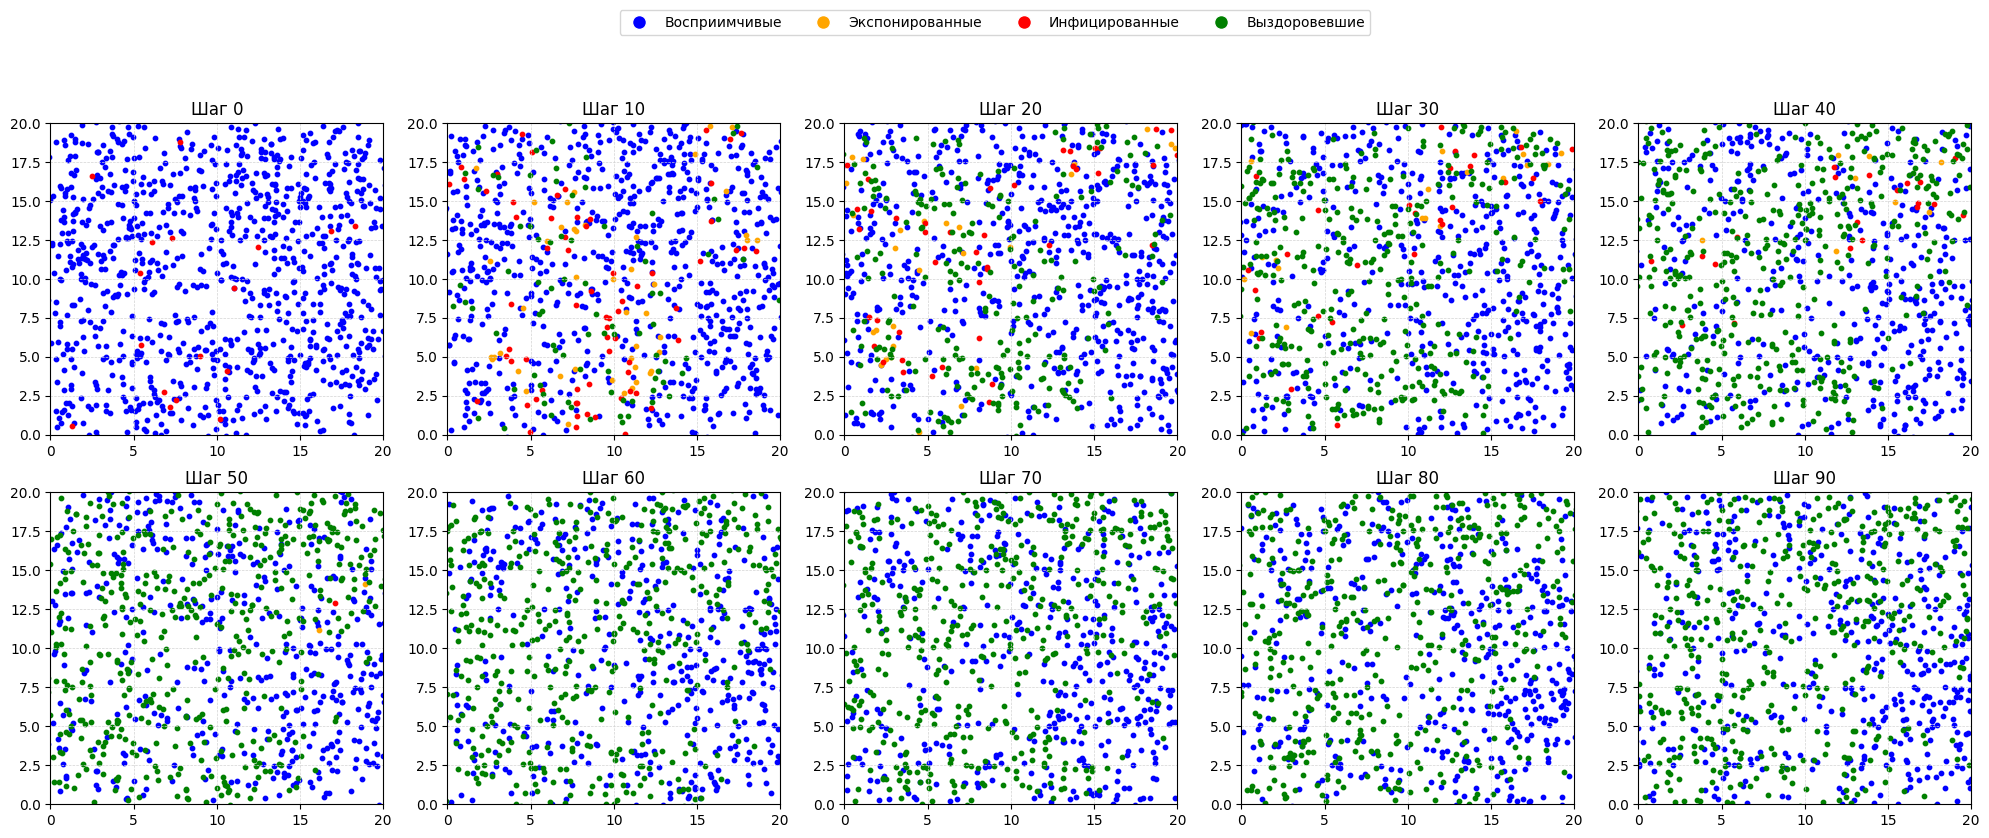
\includegraphics[scale=0.3]{images/graph04}}
		
		\dfig{Графическое представление реализации мультиагентной SEIR модели}\label{graph04}
	\end{figure}
	
	Таким образом, можно заметить, что теперь процесс распространения гриппа протекает иначе. Основной пик был между 10-ым и 20-ым днями, а далее после 60-го дня грипп не распространялся, то есть распространение прекратилось. Можно сделать выводы, что наличие у каждого индивида особых собственных свойств сильно сказывается на процессе распространения заболевания.
	
	
	\chapter*{ЗАКЛЮЧЕНИЕ}\addcontentsline{toc}{section}{ЗАКЛЮЧЕНИЕ}
	В дипломной работе была рассмотрена задача моделирования процесса распространения гриппа в условии Республики Беларусь. Для исследуемой задачи была рассмотрена SEIR-модель и ее расширения, с помощью которых был смоделирован процесс распространения заболеваний. Был проведен анализ построенных моделей и результатов симуляций процессов заболеваний. 
	
	Результаты исследований были проиллюстрированы численными экспериментами для полученных дифференциальных моделей. 
	
	В ходе работы
	\begin{enumerate}
		\item рассмотрены расширения базовой SEIR модели: вероятностная модель, пространственная модель, мультиагентная модель;
		\item на практике были рассмотрены способы построения расширений для модели SEIR для решения задачи о моделировании распространения гриппа и приведены результаты моделирования.
	\end{enumerate}
	
	С помощью рассмотренных моделей можно в дальнейшем проводить исследования по более серьезным заболеваниям. Таким образом, развитие моделей распространения заболеваний их модификаций вносит вклад в развитие имитационного моделирования.
	
	
\end{document}